\begin{figure}
\begin{fullwidth}
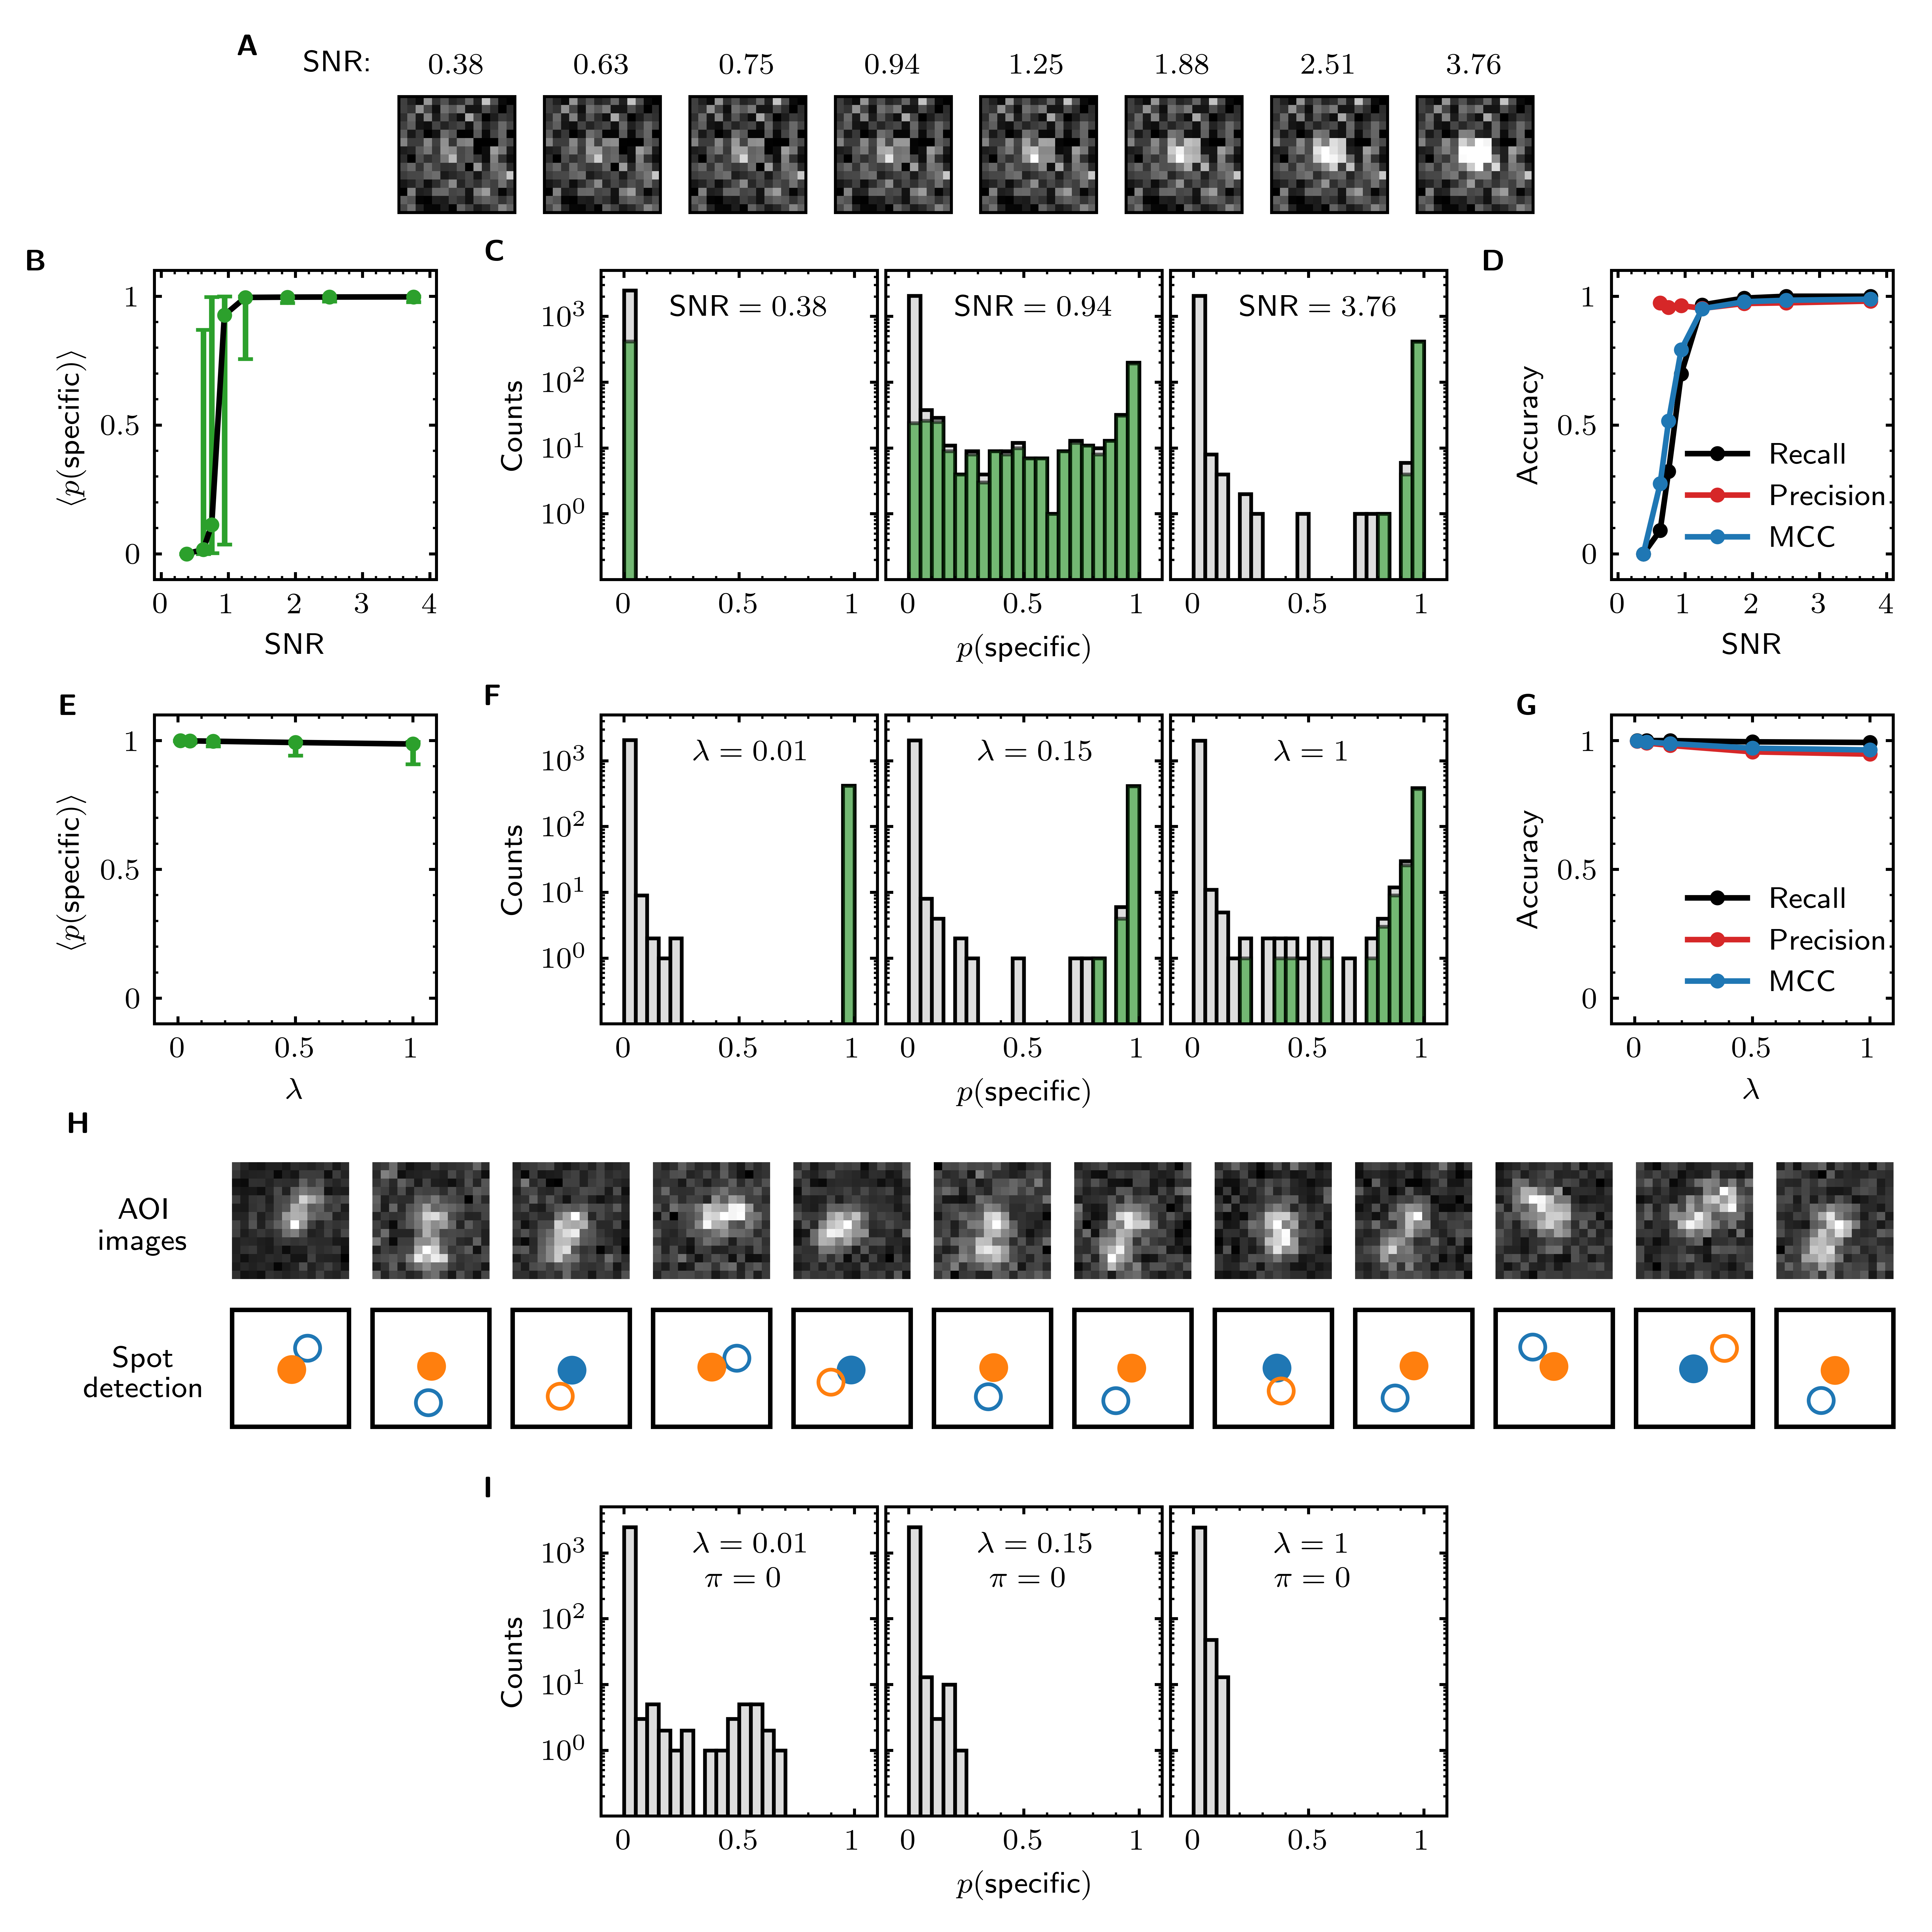
\includegraphics[width=183mm]{figures/tapqir_performance.png}
\caption{\textbf{Tapqir performance on simulated data with different SNRs or different non-specific binding rates.} (\textbf{A-D}) Analysis of simulated data over a range of SNR. SNR was varied in the simulations by changing spot intensity  $h$ while keeping other parameters constant (Supplemental Data 3). (\textbf{A}) Example images showing the appearance of the same target-specific spot simulated with increasing SNR.   (\textbf{B}) Mean of Tapqir-calculated target-specific spot probability $p(\mathsf{specific})$ (with 95\% high-density region; see Methods) for the subset of images where target-specific spots  are known to be present. (\textbf{C}) Histograms of $p(\mathsf{specific})$ for selected simulations with SNR indicated. Data are shown as stacked bars for images known to have (green, 15\%) or not have (gray, 85\%) target-specific spots.  Count is zero for bins where bars are not shown. (\textbf{D}) Accuracy of Tapqir image classification with respect to presence/absence of a target-specific spot. Accuracy was assessed by MCC, recall, and precision (see Text and Methods). (\textbf{E-G}) Same as in (\textbf{B-D}) but for the data simulated over a range of non-specific binding rates $\lambda$ at fixed SNR = 3.76 (Supplemental Data 1). (\textbf{H}) Spot recognition in AOI images containing closely spaced target-specific and non-specific spots.  Images were selected from the $\lambda = 1$ data set in e-g. AOI images and spot detection are plotted as in \FIG{tapqir_analysis}, with spot numbers 1 (blue) and 2 (orange) assigned arbitrarily and spots predicted to be target-specific shown as filled circles. (\textbf{I}) Same as in (\textbf{C}) but for the data simulated over a range of non-specific binding rates $\lambda$ with no target-specific binding ($\pi = 0$) (Supplemental Data 4).}
\label{fig:tapqir_performance}
\figsupp[False negative misidentifications by Tapqir and spot-picker method.]{\textbf{False negative misidentifications by Tapqir and spot-picker method.} The same $\lambda = 1$ simulated data set used in \FIG{tapqir_performance}e-h (\texttt{lamda1} in Supplemental Data 1) was analyzed by Tapqir and spot-picker.  The data set contained 418 AOI images containing target-specific spots, of which the 37 shown here were falsely predicted to contain no target-specific spot (3 by Tapqir and 34 by spot-picker). Correct ($+$) and incorrect ($-$) predictions by each program are indicated. In all AOI images except AOI 3 frame 109, there is a nearby target-nonspecific spot in addition to the target-specific one. False negative classifications by spot-picker method are presumably due to the presence of a closely located target-nonspecific spot that distorts the shape of a target-specific spot. Tapqir, on the other hand, is able to correctly infer the presence of two closely located spots even when they are not completely resolved (\FIG{tapqir_performance}h). The rare (3 out of 418) false negative classifications by Tapqir likely arise from target-specific spots with centers that deviate from the target location by much more ($\sim 0.7$ pixels) than the inferred proximity parameter ($\sigma^{xy} = 0.2$ pixels).}{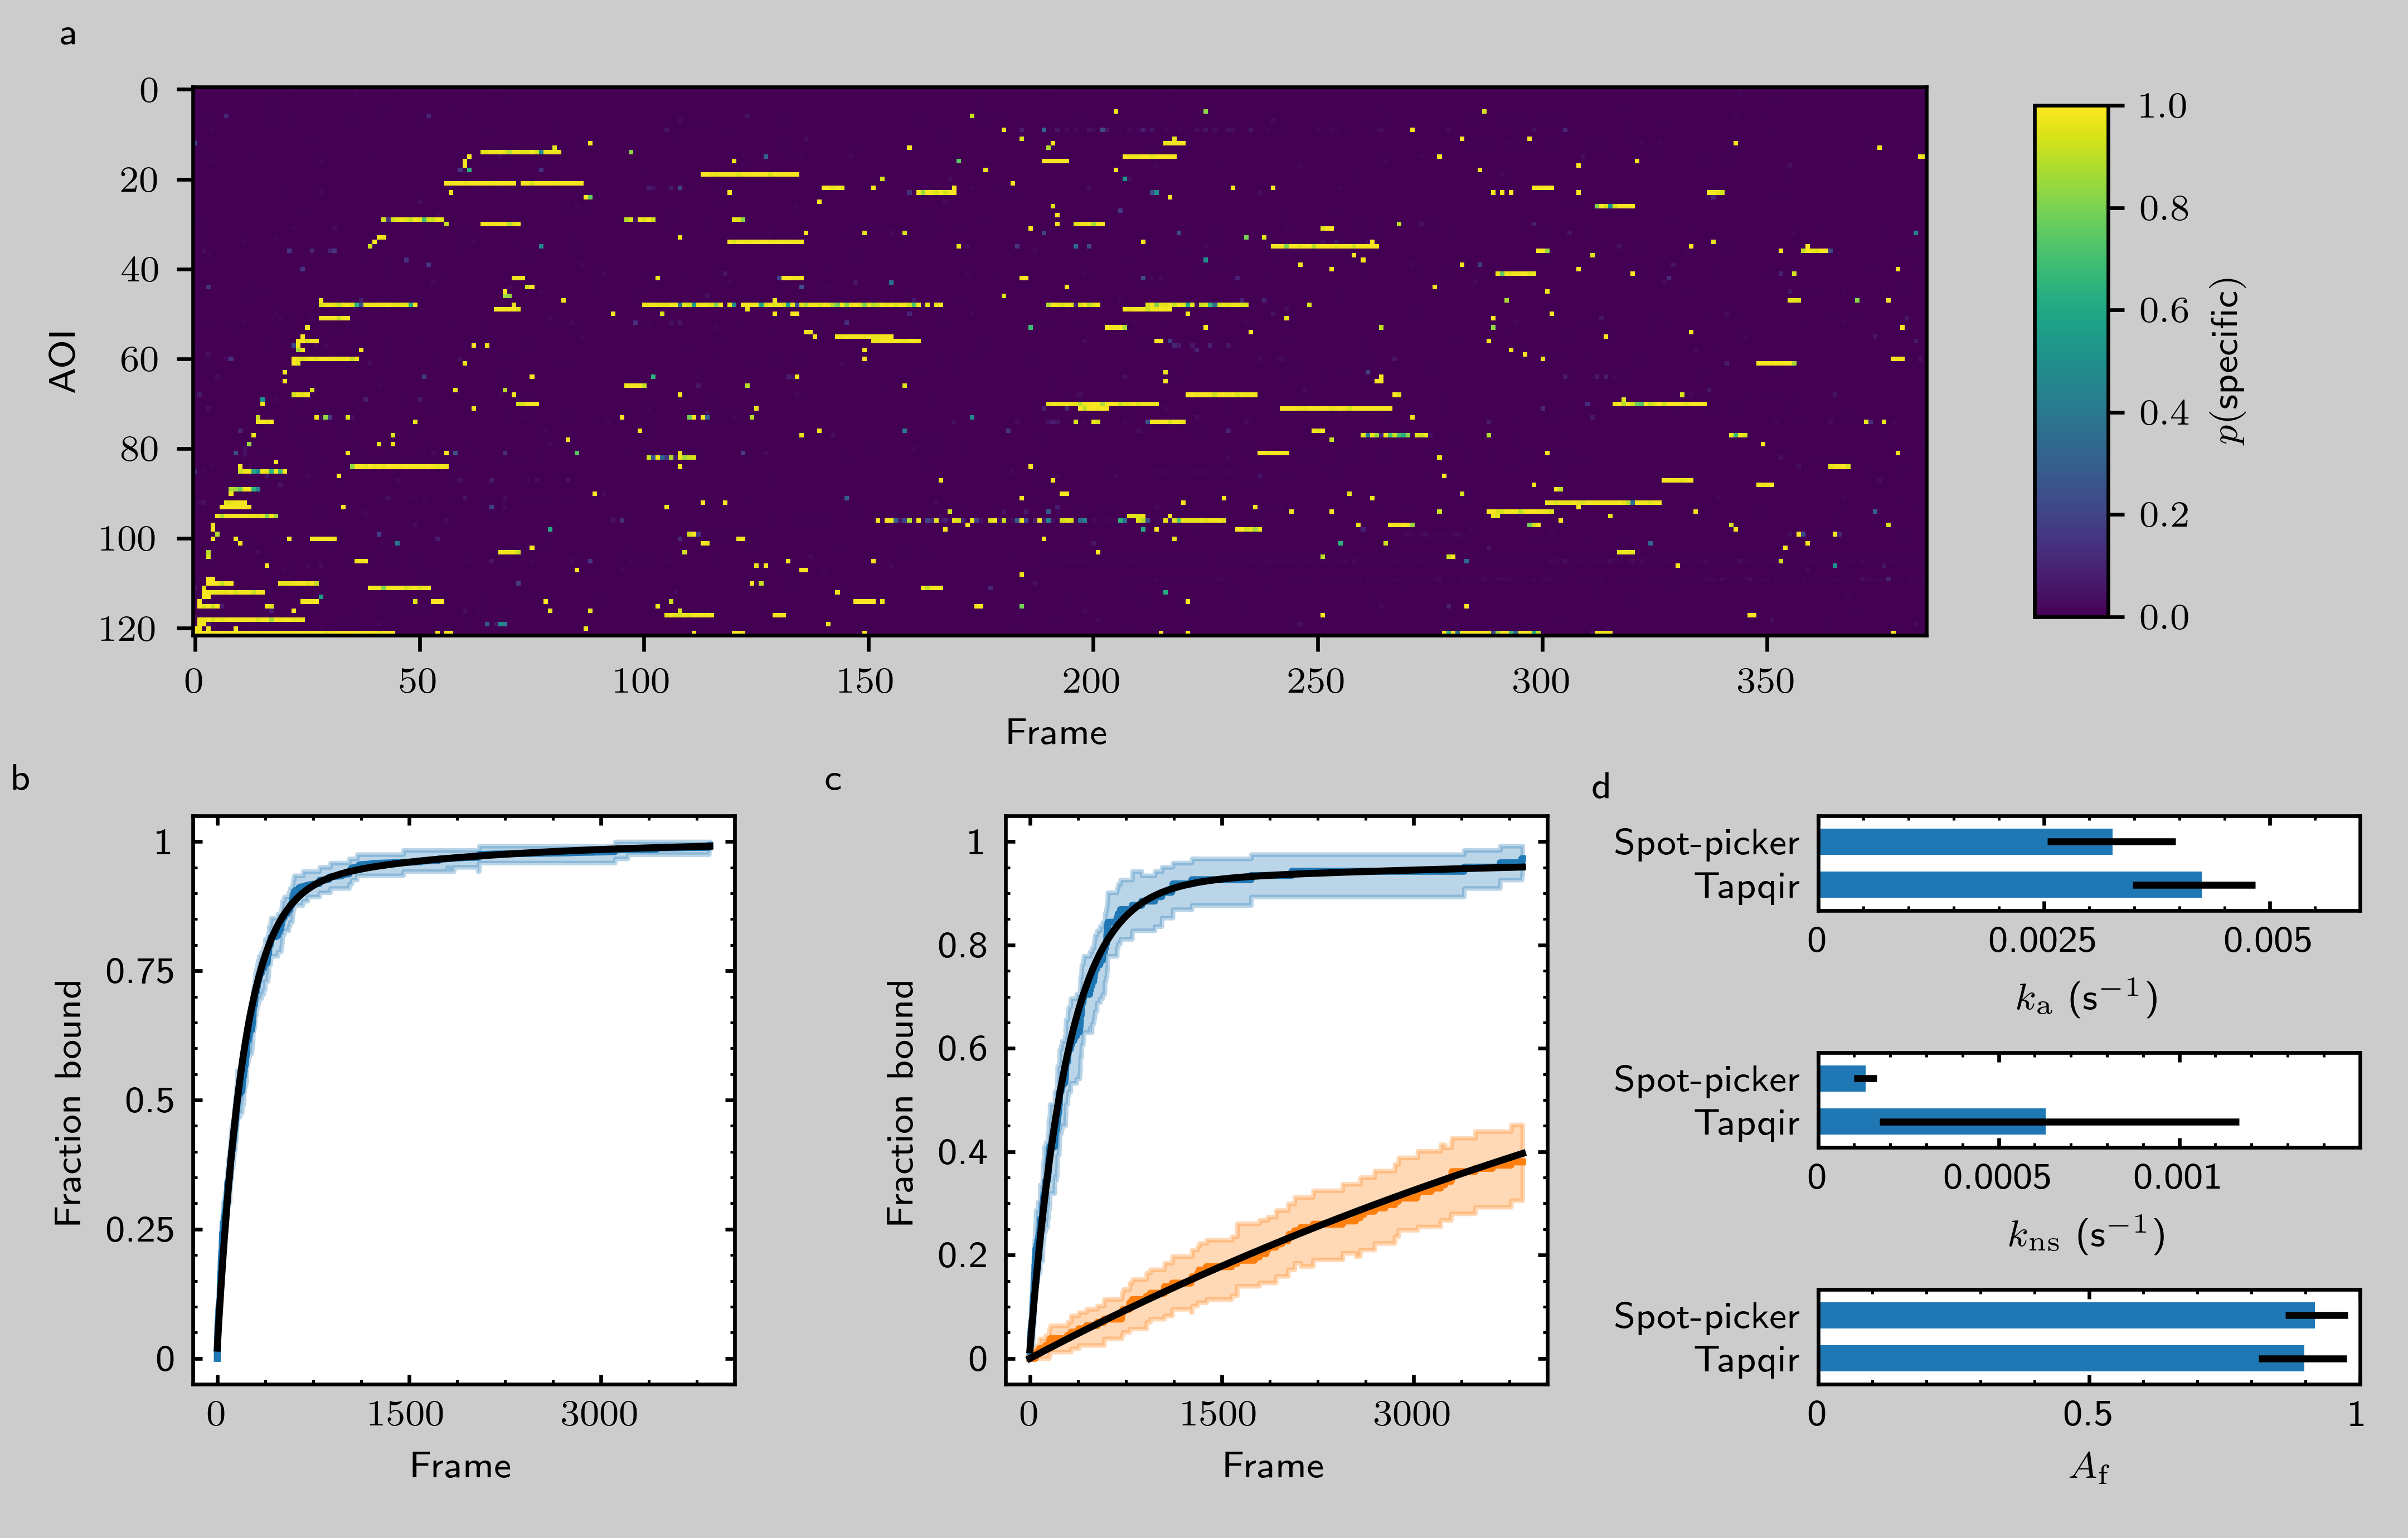
\includegraphics[width=183mm]{extended-data/figure5.png}}\label{figsupp:fn}
\end{fullwidth}
\end{figure}